%!TEX root = ../../../super_main.tex
\subsection{Consistent Dialogs}
\label{sec:consistent_dialogs}

The pop-up dialogs have undergone a major overhaul during the second sprint. The previously implemented dialog(\androidinline{GDialog} see \figref{fig:gdialog}) was found to be inconsistent with the \giraf design manual. The overall idea was that all dialogs, across the \giraf-software suite, should be replaced with standard dialogs in order the give a consistent experience. 

\begin{figure}[!htbp]
    \centering
    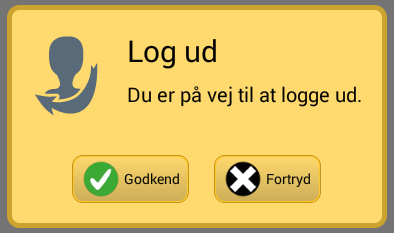
\includegraphics[width=0.4\textwidth]{sprint_two/giraf_components/gdialog}
    \caption{A GirafConfirmDialog}
    \label{fig:gdialog}
\end{figure}

\subsubsection{Design}

We found the there was two common types of dialogs where we could provide a default implementation for convenience. The first being a simple notification dialog called \androidinline{GirafNotifyDialog} which includes a title, a message, and a button for closing the dialog. And the second a confirmation dialog called \androidinline{GirafConfirmDialog} (see \figref{fig:giraf_confirm_dialog}) which provides an extra confirmation button and the possibility to provide an action for that button through an interface which the calling activity must implement. 

\begin{figure}[!htbp]
    \centering
    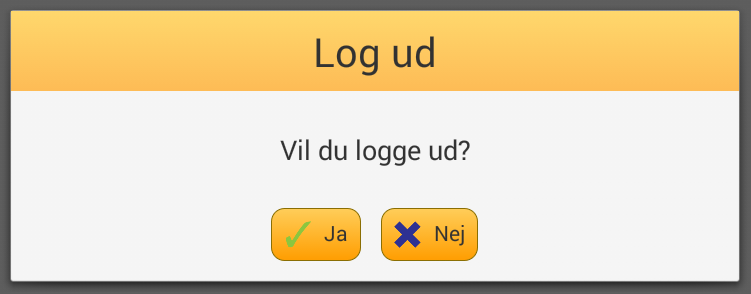
\includegraphics[width=0.7\textwidth]{sprint_two/giraf_components/giraf_confirm_dialog}
    \caption{A GirafConfirmDialog}
    \label{fig:giraf_confirm_dialog}
\end{figure}

We also provide a dialog called \androidinline{GirafCustomButtonsDialog} for simple dialog with more than two buttons.

For more specialized dialog we provide a more customizable dialog called \androidinline{GirafInflatableDialog} which inflates a given layout resource, parsed as a parameter, for the dialog.

All of the dialogs can be closed by clicking outside the dialog.

\subsubsection{Implementation}

All dialogs should ideally look similar to provide a consistent experience. This was achieved by letting all dialogs inherit from the same abstract class called \androidinline{GirafDialog} which implements functionality and visuals used in all the subclasses.

